\documentclass[11pt,letterpaper]{article}
\usepackage[margin=1in]{geometry}
\usepackage[T1]{fontenc}
\usepackage{lmodern}
\usepackage{microtype}
\usepackage{graphicx}
\usepackage{amsmath,amssymb}
\usepackage{booktabs,array}
\usepackage[numbers,sort&compress]{natbib}
\usepackage[font=small,labelfont=bf]{caption}
\usepackage{xcolor}
\usepackage{hyperref}
\hypersetup{colorlinks=true,linkcolor=blue!45!black,citecolor=blue!45!black,urlcolor=blue!45!black,
  pdftitle={Crop history, vegetation timing, and soil moisture across the U.S. Corn Belt},
  pdfauthor={Diego Osborn, Sardor Sobirov, Ivan Xie, Kyle Choi}}
\setlength{\parindent}{1.2em}
\setlength{\parskip}{0.2em}
\setlength{\emergencystretch}{1.5em}
\renewcommand{\topfraction}{0.9}
\renewcommand{\bottomfraction}{0.8}
\renewcommand{\textfraction}{0.1}
\renewcommand{\floatpagefraction}{0.75}
\setlength{\bibsep}{2pt}
\renewcommand{\bibfont}{\small}
\newcommand{\phenologyfigure}{%
\begin{figure}[htbp]
\centering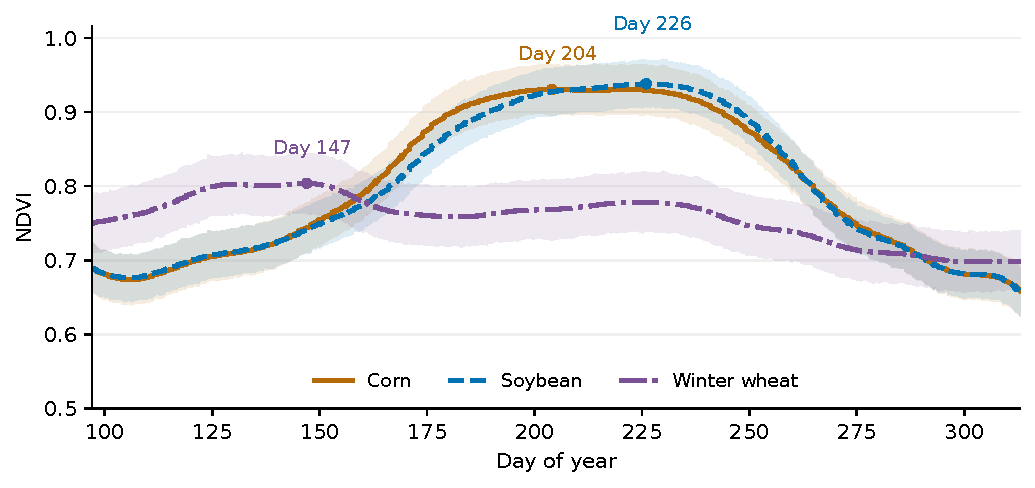
\includegraphics[width=\linewidth]{rewrite/figures/phenology.pdf}
\caption{Regional seasonal NDVI curves fitted to pooled crop--week spatial means. Lines show posterior mean curves; shading spans the 5th--95th predictive percentiles. The bands describe variation in regional means, not the spatial spread among fields. Peak labels refer to the fitted mean. The displayed window excludes winter wheat's preceding autumn growth.}
\label{fig:phenology}
\end{figure}}
\newcommand{\rotationfigure}{%
\begin{figure}[htbp]
\centering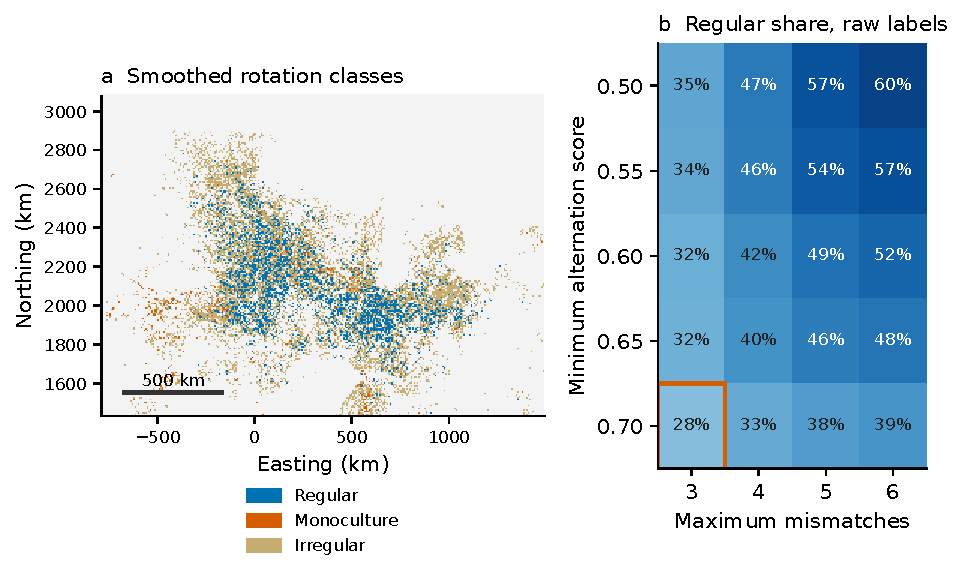
\includegraphics[width=\linewidth]{rewrite/figures/rotation.pdf}
\caption{Crop-history classes and their sensitivity to the rule. (a) The smoothed 2015--2024 map covers 2,084,112 eligible cells in the enclosing raster footprint, including cells outside the 13 state polygons. Spacing is 556.7\,m (NAD83 / Conus Albers, EPSG:5070); gray marks excluded cells. (b) The regular share before smoothing changes with the alternation and template-distance thresholds. The outlined cell marks the primary rule. Eligibility and monoculture settings remain fixed.}
\label{fig:rotation}
\end{figure}}
\title{Crop history, vegetation timing, and soil moisture\\across the U.S. Corn Belt}
\author{Diego Osborn \quad Sardor Sobirov \quad Ivan Xie \quad Kyle Choi\\[3pt]
\small Hal{\i}c{\i}o{\u g}lu Data Science Institute, UC San Diego}
\date{}
\begin{document}
\maketitle

\begin{abstract}
Annual crop maps, seasonal vegetation, and soil moisture describe different parts of an agricultural landscape. We examined their roles in a region covering 13 U.S. Corn Belt states through four complementary analyses. Smoothed regional NDVI curves separated winter wheat's early peak from the later peaks of corn and soybean. A rule-based analysis of ten-year crop histories labeled 27.36\% of 2.08 million eligible grid cells as regular corn--soybean rotation, with substantial sensitivity to the rule's thresholds. Weekly moisture percentiles described broadly wet conditions in the selected 2019 window and more geographically uneven dryness in 2022. Finally, a classifier combining crop history with concurrent seasonal observations achieved 79.21\% agreement with CDL labels on a balanced 2023 test sample. In the 2022 validation comparison, NDVI improved accuracy over crop history by 1.74 percentage points, while SMAP added little. These results support seasonal vegetation as a useful complement to crop history. Their interpretation is bounded by regional aggregation, retrospective reference periods, and unresolved feature-construction differences between training and test data.
\end{abstract}

\section{Introduction}
\label{sec:introduction}
An annual crop map records what grew where. A vegetation time series adds when the canopy developed, and soil moisture describes part of the environment in which it grew. Reading these sources together can help distinguish persistent crop patterns from seasonal changes. The practical question is which information each source adds, and how much that addition improves crop mapping.

Previous studies have used MODIS vegetation time series to distinguish crop types \citep{wardlow2007modis} and historical crop maps to predict subsequent planting \citep{zhang2019cropprediction}. Our project brings these two perspectives together with soil-moisture summaries. It examines four questions: how seasonal vegetation differs among crops, how often corn--soybean histories follow a repeated sequence, where surface moisture departs from its seasonal reference, and whether current-season observations improve classification beyond crop history.

The first three analyses describe regional patterns; the fourth tests how seasonal observations add to classification based on crop history. Agricultural resilience motivates the work, but the study does not measure yield losses, recovery, or the effects of management decisions.

\section{Data and study design}
\label{sec:data}
The study covers Illinois, Indiana, Iowa, Kansas, Kentucky, Michigan, Minnesota, Missouri, Nebraska, North Dakota, Ohio, South Dakota, and Wisconsin. We used three data streams: annual USDA Cropland Data Layer (CDL) labels, weekly MODIS normalized difference vegetation index (NDVI) composites, and weekly SMAP Level-4 surface soil moisture. CDL supplies the crop categories \citep{cdl_cropscape}; NDVI summarizes canopy greenness \citep{modis_vi_userguide}; and SMAP L4 combines observations with a land-surface model to estimate moisture \citep{reichle2017smap}. NDVI and SMAP composites were accessed through CropSmart.

The analyses use different time windows (Table~\ref{tab:design}). For vegetation, the workflow retains approximately day of year 100--310, covering spring through autumn. Moisture references use matching ISO weeks for the selected event windows. Crop masks follow annual CDL labels, except where the classifier uses a fixed eligible footprint and balances the target classes during sampling.

Raster downloads use a buffered rectangle enclosing the study states. Whole-raster summaries therefore include eligible cells outside their boundaries: the rotation output assigns 66,107 of its 2,084,112 cells (3.17\%) to \texttt{outside\_configured\_states}. We retain that footprint for the overall rotation shares and restrict named-state moisture summaries to their assigned state groups.

\begin{table}[htbp]
\centering\small
\begin{tabular}{>{\raggedright\arraybackslash}p{0.20\linewidth}>{\raggedright\arraybackslash}p{0.31\linewidth}>{\raggedright\arraybackslash}p{0.40\linewidth}}
\toprule
Analysis & Time window & Unit and main output \\
\midrule
Seasonal signatures & 2008--2025, available weeks & Crop--week regional means; one pooled curve per crop \\
Crop histories & 2015--2024 & Eligible grid cell; rule-based sequence class \\
Moisture conditions & Reference: 2015--2021; events: Apr--Jul 2019 and Jun--Aug 2022 & Cell--week scores; state--crop summaries \\
Crop classification & Train: 2013--2021; validation: 2022; test: 2023 & Balanced cell--year sample; current-year CDL class \\
\bottomrule
\end{tabular}
\caption{Analysis windows and units. The classifier uses preceding crop history and current-season observations; the event analysis includes 2019 in its reference period.}
\label{tab:design}
\end{table}

The processing workflow requests rasters in NAD83 / Conus Albers (EPSG:5070), stores them as indexed tables, and joins sources by grid coordinates. Source resolution and analysis spacing must be distinguished. Historical CDL is commonly described at 30\,m, the MODIS vegetation product at 250\,m, and SMAP L4 at 9\,km. The saved rotation raster records 556.7\,m spacing on a $4096\times2960$ grid. That spacing is verified for this output. Resampling cannot create finer independent moisture information. Missing metadata for some intermediate tables also leaves complete cross-product grid alignment unverified.

Figure~\ref{fig:workflow} shows how the analyses relate. CDL labels define crop groups for the vegetation and moisture summaries as well as supplying crop histories. The classifier derives its features directly from annual labels and seasonal observations. It does not ingest the fitted Gaussian-process curves, Bayesian moisture scores, or the full-period rotation map.

\begin{figure}[htbp]
\centering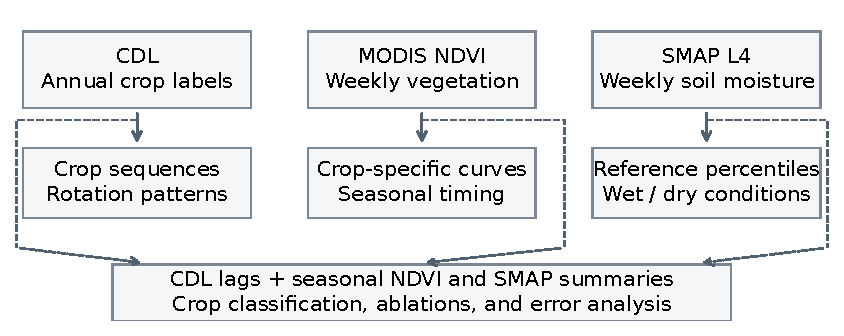
\includegraphics[width=\linewidth]{rewrite/figures/workflow.pdf}
\caption{The three data streams support descriptive analyses and a separate classification experiment. Solid arrows mark each descriptive analysis's main input; CDL also supplies its crop groupings. Dashed paths show source-derived features entering the classifier. Fitted curves and moisture scores do not feed the classifier.}
\label{fig:workflow}
\end{figure}

\section{Seasonal crop signatures}
\label{sec:phenology}

We first compared seasonal NDVI curves to see which aspects of vegetation timing distinguish the crop classes. Corn and soybean can reach similar peak greenness, so their timing and seasonal shape may be more useful than peak magnitude alone. Winter wheat provides an earlier seasonal contrast.

For each available year from 2008 to 2025, we joined weekly NDVI to that year's CDL labels and calculated the spatial mean for corn, soybean, and winter wheat (CDL codes 1, 5, and 24). We converted the weekly dates to day of year (DOY) and pooled the resulting observations by crop. Each model used 535 weekly spatial means. Annual CDL masks let a cell's crop group change from year to year.

We fitted a separate Hilbert space Gaussian process (HSGP) to each crop to obtain a smooth seasonal curve. This approximation represents the Gaussian process with a finite set of basis functions \citep{riutort2023hsgp}. Our implementation used 25 basis functions, a squared-exponential covariance, and normally distributed residuals. Variational inference estimated an approximate posterior distribution. The model pools years without estimating a separate seasonal curve for each year, so its main use here is to describe the average seasonal pattern. Predictive bands include the model's residual variation among weekly regional means.

The fitted corn curve peaks at DOY~204 with NDVI~0.930, while soybean peaks at DOY~226 with NDVI~0.938 (Figure~\ref{fig:phenology}). Their peak magnitudes are close, but soybean's modeled peak occurs 22 days later. Winter wheat peaks earlier, at DOY~147 and NDVI~0.804. These contrasts indicate why a sequence of seasonal observations can contain information that a single peak value misses. They describe the observed spring-to-autumn window; the analysis does not cover winter wheat's preceding autumn establishment.

In-sample root mean squared error was 0.0194 for corn, 0.0183 for soybean, and 0.0232 for winter wheat. The 90\% posterior predictive intervals contained 90.09--91.21\% of the weekly spatial means used for fitting. These checks describe fit to regional averages; they do not establish calibration on unseen years or precision about individual fields.

\phenologyfigure

\section{Crop-history patterns}
\label{sec:rotation}

We next examined how often annual crop labels follow a repeated corn--soybean sequence. Comparing multi-year CDL sequences is an established approach to describing rotation patterns \citep{sahajpal2014recruit}. Here we used a transparent rule to distinguish repeated alternation, persistent single-crop histories, and other sequences over 2015--2024. Cells entered the analysis if corn or soybean appeared in at least five of the ten years, leaving 2,084,112 eligible cells.

The rule combines three views of the sequence. The alternation score is the fraction of adjacent-year pairs that switch between corn and soybean, counting only pairs in which both years have one of those labels. Pairs involving other labels are excluded from this denominator. Pattern distance counts mismatched years against the closer of two fixed templates: corn--soybean alternation starting with corn, or starting with soybean. Other crop labels count as mismatches. The longest run and the largest single-crop share identify persistent cropping.

Classification applies the monoculture rule first: a cell receives that label if one crop appears for at least seven consecutive years or occupies at least eight of the ten years. Among the remaining cells, regular rotation requires an alternation score of at least 0.70, no more than three template mismatches, and at least seven corn-or-soybean years. All other eligible cells are labeled irregular. The five-year eligibility threshold therefore defines the population being described, while the seven-year requirement belongs to the stricter regular-rotation rule.

We applied a $3\times3$ majority filter to the class map to reduce isolated labels while preserving the eligible footprint. In the saved smoothed map, regular rotation accounts for 27.36\% of eligible cells, monoculture for 3.90\%, and irregular histories for 68.74\% (Figure~\ref{fig:rotation}). These shares describe the classified analysis grid. Its recorded cell spacing is approximately 556.7~m, so the map and derived areas cannot be interpreted as a field inventory or as native-resolution CDL acreage estimates. Smoothing can also change a cell's label relative to its own sequence.

Before spatial smoothing, the primary rule labels 28.15\% of cells as regular. Lowering the alternation threshold to 0.50 and allowing six template mismatches raises this share to 60.33\%, with eligibility, the seven-year corn-or-soybean requirement, and the monoculture rule unchanged. These are raw classifications of the same eligible cells. An irregular label can include a repeated multi-crop sequence, an interruption in corn--soybean alternation, or errors in annual labels; it does not establish poor management.

\rotationfigure

\section{Wet and dry soil conditions}
\label{sec:moisture}

We used weekly SMAP L4 surface soil moisture to describe departures from
usual seasonal conditions during April--July 2019 and June--August 2022,
the two event windows selected for the flood and drought case studies.
The analysis covered cells eligible for the crop-history analysis and
grouped them by state and event-year CDL label. The crop strata were corn
(1), soybean (5), winter wheat/soybean double crop (26), and oats (28).
SMAP retains its native 9~km spatial support when assigned to the finer
crop grid, so neighboring crop cells can share the same moisture
information.

For each cell and calendar week (ISO week), we estimated a reference mean
and sample standard deviation from 2015--2021, giving at most seven annual
observations. We expressed each event observation as a departure from that
mean in standard-deviation units, with stored $z$-scores clipped to
$[-5,5]$. The reference includes 2019 but precedes 2022. Including 2019
can dampen its anomaly. We treat these as retrospective case studies;
holding out both events would require excluding each event year from its
reference.

We also fitted an empirical-Bayes Normal--Inverse-Gamma model to account
for uncertainty in the reference mean and variance. Its conjugate update
gives a Student-$t$ posterior predictive distribution \citep{murphy2007conjugate}.
The prior mean was the regional mean for the corresponding week; the
variance prior used the regional median of the cell-level baseline
variances. We evaluated the predictive cumulative distribution at each
observed moisture value. This moisture
percentile approaches zero for unusually dry observations and one for
unusually wet observations. It is a position within the fitted moisture
distribution, not a probability that drought is present.

Figure~\ref{fig:moisture} compares mean moisture percentiles for corn and
soybean in each state, with a reference line at 0.5 on the zero-to-one
scale. We averaged the individual pixel-week scores within each
state--crop group and also counted fractions beyond selected thresholds.
A cell observed in several weeks contributes several times. These
fractions therefore describe the combined spatial and temporal extent of
unusual conditions within the sampled population.

The 2019 mean moisture percentiles exceeded 0.5 for corn and soybean in
every study state, reaching 0.85 for South Dakota corn. In Iowa, 17.75\% of
2,901,150 corn pixel-weeks exceeded $z=1.5$, indicating repeated or
widespread departures above the weekly reference. These elevated values
describe relative wetness; identifying flooded fields would require
separate inundation observations.

The 2022 window showed a different pattern. Nebraska soybean had a mean
moisture percentile of 0.24, and 40.54\% of its 947,648 pixel-weeks fell
below the tenth predictive percentile. North Dakota corn averaged 0.52,
showing the geographic variation in the dry signal. Kentucky's winter
wheat/soybean double-crop stratum had 41.96\% of 49,543 pixel-weeks below
the tenth percentile.
Differences among these crop strata reflect their spatial distributions
as well as the moisture conditions encountered, which limits comparisons
of crop-specific responses to water stress.

These summaries identify where and when surface moisture was unusual
within the sampled crop-history population. Read alongside seasonal NDVI,
they provide context for crop-condition monitoring.


\begin{figure}[htbp]
\centering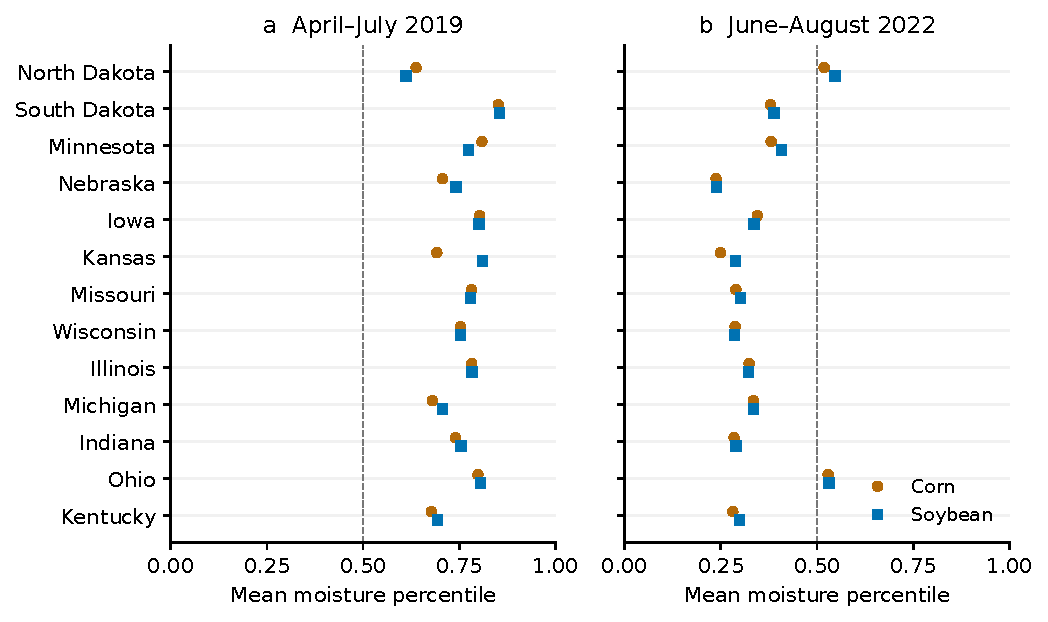
\includegraphics[width=\linewidth]{rewrite/figures/moisture.pdf}
\caption{Mean moisture percentile by state and crop during the two selected windows. Each point averages posterior predictive CDF scores over the group's cell--week rows. Lower values indicate drier conditions relative to the 2015--2021 weekly reference; higher values indicate wetter conditions. The dashed line marks the reference distribution's median percentile, not an event-detection threshold. These are summaries of the sampled crop-history footprint, not area-weighted estimates of fields affected.}
\label{fig:moisture}
\end{figure}

\section{Crop classification from history and seasonal observations}
\label{sec:classification}

\subsection{What seasonal observations add}

We tested whether current-season NDVI and soil moisture improve crop
classification beyond the information in preceding crop labels.
The target was the current year's CDL class: corn (code~1), soybean (5),
winter wheat (24), or Other. Other combines the remaining selected CDL codes
(0--61), including code~0. The experiment used concurrent observations
through late season; forecasting before planting would require an earlier
observation cutoff and a separate evaluation.

The classification mask retained cells with selected CDL codes (0--61) in
at least three years during 2013--2022, separately from the rotation
analysis's corn--soybean eligibility rule. Each sample represented a grid
cell in one year. The full model used 38
features: 19 from CDL history, 15 from NDVI, and four from SMAP. CDL features
summarized up to ten preceding years through five annual lags, corn--soybean
transition counts, crop frequencies, time since each crop, sequence metrics,
and $3\times3$ neighborhood summaries. NDVI features described the current
season's level, amplitude, peak and green-up timing, rate of green-up, and
early-, middle-, and late-season means. Four additional NDVI summaries
described historical peak magnitude and timing. These features were calculated
directly from the weekly observations. SMAP supplied spring and growing-season
means plus fractions of weeks above an 80th-percentile or below a
20th-percentile reference.

We fitted a LightGBM classifier \citep{ke2017lightgbm} with a maximum of 500
boosting rounds, learning rate 0.05, maximum tree depth seven, and 63 leaves.
Training used 4.5 million samples from 2013--2021; the 2013--2014 rows retained
missing SMAP inputs because that record begins in 2015. The 2022 validation set
controlled early stopping after 50 rounds without improvement and supported
the feature-group comparison. The full model was then evaluated on 2023.
Sampling selected 125,000 observations from each class per year, giving
500,000 observations in each held-out year. Accuracy therefore measures
agreement with CDL on a balanced sample. Estimating regional map accuracy
would require area-weighted evaluation. Macro F1 averages the four
class-specific F1 scores with equal weight.

\begin{table}[htbp]
\centering
\small
\begin{tabular}{lrrr}
\hline
Features & Number & Accuracy (\%) & Macro F1 \\
\hline
CDL history & 19 & 80.59 & 0.8080 \\
CDL + NDVI & 34 & \textbf{82.33} & \textbf{0.8245} \\
CDL + SMAP & 23 & 80.66 & 0.8086 \\
CDL + NDVI + SMAP & 38 & 82.26 & 0.8239 \\
\hline
\end{tabular}
\caption{Feature-group comparison on the balanced 2022 validation sample
($n=500{,}000$). All configurations used the same training and validation
years. These are validation results, not comparisons on the 2023 test set.}
\label{tab:ablation}
\end{table}

NDVI produced the largest improvement over crop history
(Table~\ref{tab:ablation}): accuracy increased by 1.74 percentage points.
Winter wheat showed the largest class-specific gain, with F1 rising from
0.849 to 0.881. This is consistent with the earlier seasonal peak seen in
the separate phenology analysis, although the comparison does not isolate
which NDVI feature caused the gain. Adding SMAP to CDL alone increased
accuracy by 0.07 percentage points. The full model scored slightly below
CDL plus NDVI. These observed differences support NDVI's value in this
validation year; they do not establish statistical significance or the same
ordering in other years.

\subsection{Test-year errors and crop-history patterns}

The full model achieved 79.21\% accuracy and 0.7914 macro F1 in 2023
(Figure~\ref{fig:prediction}). F1 was 0.893 for Other, 0.813 for
winter wheat, 0.726 for corn, and 0.735 for soybean. The largest individual
confusion was soybean classified as corn: 30,935 of the 125,000 soybean
samples, compared with 9,894 corn samples classified as soybean. The model
therefore retained substantial confusion between the two summer crops
despite the additional seasonal observations.

To examine performance across crop histories, the feature builder assigned
regimes using each target year's preceding historical window. These are
separate from the 2015--2024 rotation map. A regular history required an
alternation score of at least 0.7 and a distance of at most three from a
canonical corn--soybean sequence. Monoculture took precedence when the
longest repeated-crop run reached seven years or the corn or soybean
fraction reached 0.8; remaining histories were labeled irregular.

Accuracy was 95.55\% for monoculture histories ($n=124{,}318$), 87.41\% for
regular rotation ($n=65{,}574$), and 70.92\% for irregular histories
($n=310{,}108$). Different class mixtures across these groups prevent a
causal interpretation of the accuracy gaps. The regular group's high accuracy
also masks uneven performance across classes: corn and soybean F1 scores were
0.879 and 0.907, while four-class macro F1 was 0.559.

\subsection{Interpreting the fitted model}

To examine which inputs influenced the fitted model, we applied SHAP
TreeExplainer \citep{lundberg2017shap} to a random sample of 1,000 test
observations. Mean absolute attribution ranked the previous
year's CDL code first, followed by mid-season NDVI, NDVI peak timing, and
late- and early-season NDVI means. Growing-season mean soil moisture ranked
eighth. These rankings describe the fitted model's use of its inputs.


\begin{figure}[htbp]
\centering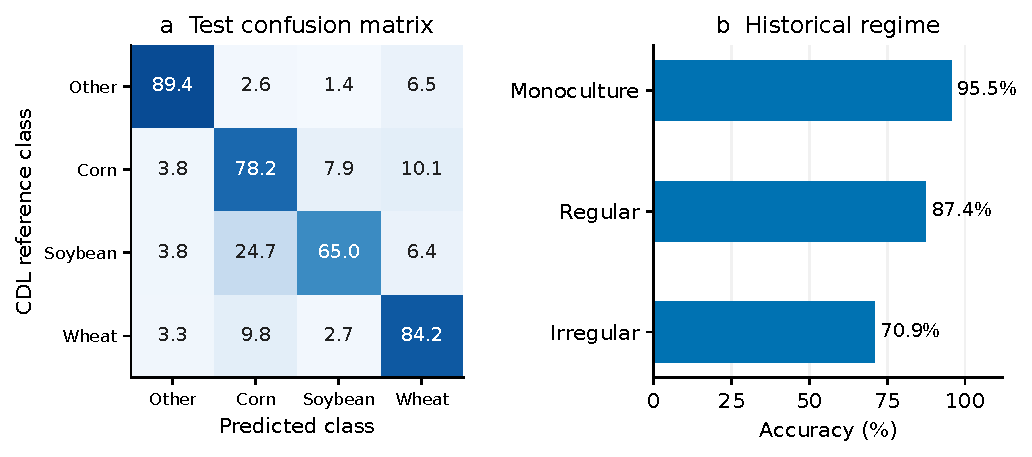
\includegraphics[width=\linewidth]{rewrite/figures/prediction.pdf}
\caption{Full-model results for the balanced 2023 test sample. (a) Confusion-matrix entries are row percentages; each CDL reference class contains 125,000 samples. Wheat denotes winter wheat (code~24); Other combines the remaining selected CDL labels. (b) Accuracy differs across regimes assigned from preceding crop history. The groups have different class mixtures, so their accuracy gaps do not isolate the effect of rotation complexity.}
\label{fig:prediction}
\end{figure}

\section{What the combined results support}
\label{sec:discussion}
Seasonal NDVI has the clearest measured value for crop classification in this study. Its improvement over crop history agrees with the distinct timing seen in the regional curves, although the experiment does not identify which timing feature accounts for the gain. Crop history remains a useful baseline, but its interpretation depends on the sequence rule and the crop classes represented. The rotation sensitivity and errors by regime therefore point to the need to evaluate performance across crop histories, with class composition reported alongside accuracy.

The moisture analysis serves a different purpose: it describes departures from usual seasonal conditions. The small classification gain from the selected SMAP features applies to that feature set and validation year. Evaluating moisture for crop-condition monitoring would require a defined outcome and an evaluation designed around it.

\subsection{Limits of the evidence}
Three issues matter for interpreting or extending these results. First, the units are coarser than individual fields. Regional NDVI averages hide local variability, resampled moisture cells share information, and annual CDL errors can alter apparent crop sequences. Model agreement with CDL therefore measures consistency with a reference product, not independent field accuracy. A spatially separated evaluation would be needed to assess transfer to new locations \citep{roberts2017cv}.

Second, the current classifier's feature construction is not fully consistent across splits. Neighborhood summaries are built after target-class sampling, with unsampled locations filled as zero; consequently, the sampling process can influence predictors. Historical NDVI summaries also have different observation coverage in training and test construction. For SMAP, training uses historical percentile references when available, while the test builder falls back to the current row's seasonal percentiles. In addition, the fixed eligible mask uses 2013--2022 labels, including years later than some training samples. These findings warrant a common feature builder with explicit time cutoffs and a repeat evaluation before deployment. We have not measured their effect on the reported scores.

Third, the moisture comparison is retrospective and uses a short reference period. The inclusion of 2019 in that reference can attenuate its anomalies. Neither event analysis has independent labels for flood extent, drought severity, or crop damage, so the scores describe unusual moisture rather than validated detection performance. A prospective study would require a reference ending before each event and outcome data suited to the intended claim.

\section{Conclusion}
Seasonal NDVI added more to classification based on crop history than the selected soil-moisture features in the reported validation comparison. The descriptive analyses help interpret these inputs while showing the limits imposed by aggregation and classification rules. The next test is to construct features consistently at explicit time cutoffs and evaluate them across years and unseen locations. Moisture monitoring needs its own crop-condition outcome and validation data.

\section*{Code and reproducibility}
Code, notebooks, and saved results are available in the \href{https://github.com/sardorsob/GeoCrop-Spatiotemporal-Modeling}{GeoCrop repository}. This revision redraws figures from saved results without refitting models. Build instructions and figure-source checksums are in \texttt{artifacts/reports/rewrite/}. Recreating the analyses also requires the downloaded input data and their spatial metadata.

\raggedright
\bibliographystyle{unsrtnat}
\bibliography{references_revised}
\end{document}
